We have been writing the missing manual for peer-produced peer
learning -- the ``Peeragogy Handbook''
(\href{http://peeragogy.org/}{peeragogy.org}).  While building this
book, we,~ourselves peer learners in this quest,~have been mindful of
these four questions:

\begin{enumerate}
\itemsep1pt\parskip0pt\parsep0pt
\item
  \emph{How does a motivated group of self-learners choose a subject or
  skill to learn?~}
\item
  \emph{How can this group identify and select the best learning
  resources about that topic?~}
\item
  \emph{How will these learners identify and select the appropriate
  technology and communications tools and platforms to accomplish their
  learning goal?}
\item
  \emph{What does the group need to know about learning theory and
  practice to put together a successful peer-learning program?}
\end{enumerate}

It is clear to us that the techniques of peer production that have built
and continue to improve \emph{Wikipedia} and GNU/Linux have yet to fully
demonstrate their power in education. We believe that the
\emph{Peeragogy Handbook} can help change that by building a distributed
community of peer learners/educators, and a strongly vetted collection
of best practices. Our project complements others' work on sites like
Wikiversity and P2PU, and builds upon understandings that have
developed informally in distributed communities of hobbyists and
professionals, as well as in (and beyond) the classrooms of
generations of passionate educators. Here, we present Peeragogy in
Action, a project guide in four parts. Each part relates to one or
more sections of our handbook, and suggests activities to try while
you explore peer learning. These activities are designed for flexible
use by widely distributed groups, collaborating via a light-weight
infrastructure. Participants may be educators, community organizers,
designers, hackers, dancers, students, seasoned peeragogues, or
first-timers. The guide should be useful for groups who want to build
a strong collaboration, as well as to facilitators or theorists who
want to hone their practice or approach.  Together, we will use our
various talents to build effective methods and models for peer
produced peer learning. Let's get started!


\noindent\raisebox{-2.7in}{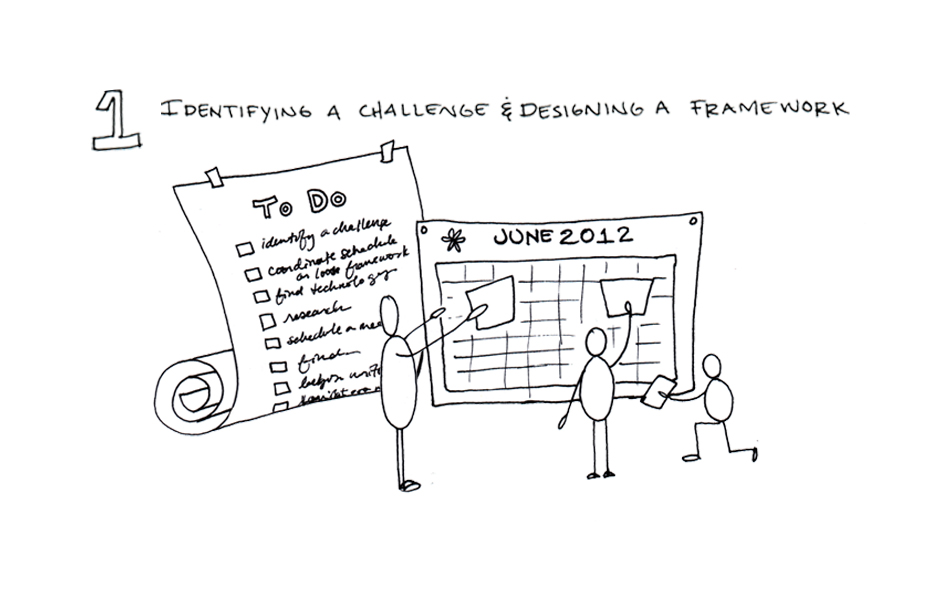
\includegraphics[width=.25\textwidth]{../pictures/OpenBook-2-1.jpg}}

\textbf{Setting the initial challenge and building a framework for
accountability among participants is an important starting point.}

\emph{Activity} -- Come up with a plan for your work and an agreement,
or informal contract, for your group. You can use the suggestions in
this guide as a starting point, but your first task is to revise the
plan to suit your needs. It might be helpful to ask: What are you
interested in learning? What is your primary intended outcome? What
problem do you hope to solve? ~How collaborative does your project need
to be? How will the participants' expertise in the topic vary? What sort
of support will you and other participants require? What problems won't
you solve?

\emph{Technology} -- Familiarize yourself with the collaboration tools
you intend to use (e.g.~WordPress, Git and LaTeX, YouTube, GIMP, a
public wiki, a private forum, or something else) and create a first
post, edit, or video introducing yourself and your project(s) to others
in the worldwide peeragogy community.

\emph{Suggested Resources} -- The Peeragogy Handbook, parts I
(`\href{http://peeragogy.org/}{Introduction}') and II
(`\href{http://peeragogy.org/motivation/}{Motivation}'). You may
also want to work through a short lesson called
\href{https://en.wikiversity.org/wiki/User:Arided/ImplementingParagogy}{Implementing
Paragogy},~from the early days before the Peeragogy project was
convened. For a succinct theoretical treatment, please refer to our
literature review, which we have adapted into a
\href{http://en.wikipedia.org/wiki/Peer_learning}{Wikipedia page}.

\emph{Further Reading} -- Boud, D. and Lee, A. (2005). \emph{`Peer
learning' as pedagogic discourse for research education}. Studies in
Higher Education, 30(5):501--516.

\emph{Observations from the Peeragogy project} -- We had a fairly weak
project structure at the outset, which yielded mixed results. One
participant said: ``I definitely think I do better when presented with a
framework or scaffold to use for participation or content development.''
Yet the same person wrote with enthusiasm about models of
entrepreneurship, saying she was ``freed of the requirement or need for
an entrepreneurial visionary.'' 

\noindent\raisebox{-2.7in}{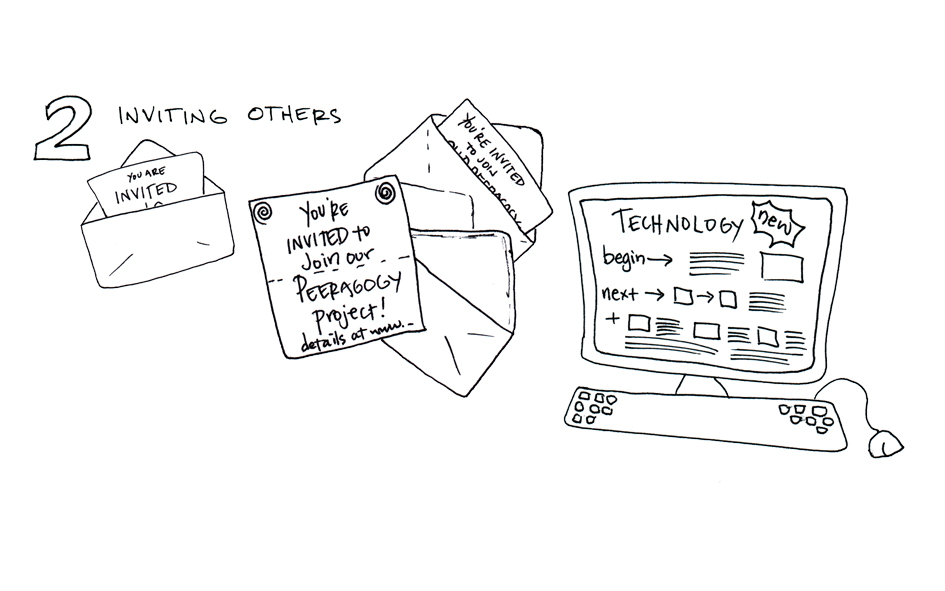
\includegraphics[width=.25\textwidth]{../pictures/OpenBook-2-2.jpg}}

\textbf{Other people can support you in achieving your goal and make the
work more fun too.}

\emph{Activity} -- Write an invitation to someone who can help as a
co-facilitator on your project. Clarify what you hope to learn from them
and what your project has to offer. Helpful questions to consider as you
think about who to invite: What resources are available or missing? What
do you already have that you can build on? How will you find the
necessary resources? Who else is interested in these kinds of
challenges? Go through the these questions again when you have a small
group, and come up with a list of more people you'd like to invite or
consult with as the project progresses.

\emph{Technology} -- Identify tools that could potentially be useful
during the project, even if it's new to you. Start learning how to use
them. Connect with people in other locales who share similar interests
or know the tools.

\emph{Suggested resources} -- The Peeragogy Handbook, parts IV
(`\href{http://peeragogy.org/convening-a-group/}{Convening a Group}')
and V
(`\href{http://peeragogy.org/organizing-a-learning-context/}{Organizing
a Learning Context}').

\emph{Recommended Reading} -- Schmidt, J. Philipp. (2009). Commons-Based
Peer Production and education. Free Culture Research Workshop Harvard
University, 23 October 2009.

\emph{Observations from the Peeragogy project} -- We used a strategy of
``open enrollment.'' New people were welcome to join the project at any
time. We also encouraged people to either stay involved or withdraw;
several times over the first year, we required participants to
explicitly reaffirm interest in order to stay registered in the forum
and mailing list.

\noindent\raisebox{-2.7in}{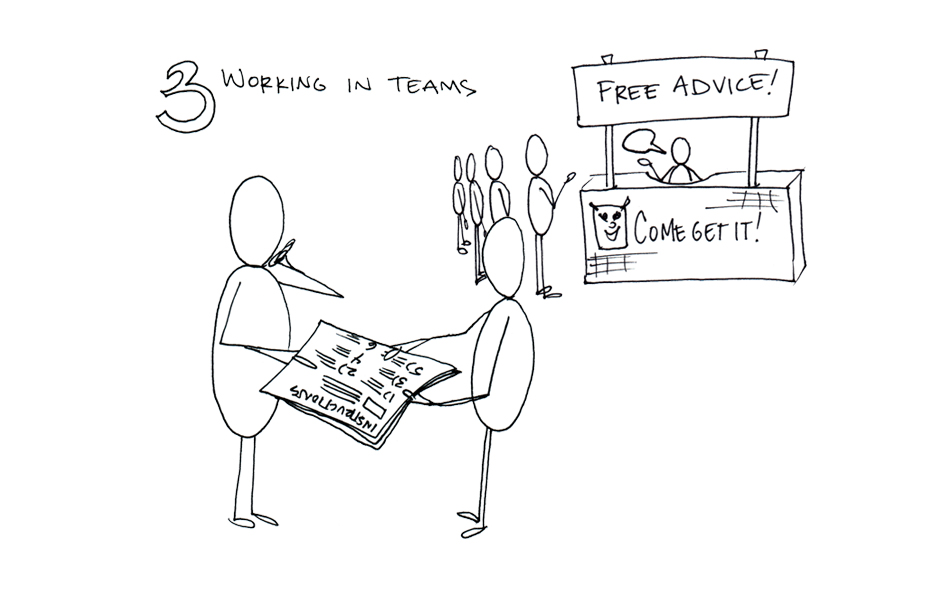
\includegraphics[width=.25\textwidth]{../pictures/OpenBook-2-3.jpg}}

\textbf{Solidifying your work plan and learning strategy together with
concrete measures for `success' can move the project forward
significantly.}

\emph{Activity} -- Distill your ideas by writing an essay, making visual
sketches, or creating a short video to communicate the unique plans for
organization and evaluation that your group will use. By this time, you
should have identified which aspects of the project need to be refined
or expanded. Dive in!

\emph{Technology} -- Take time to mentor others or be mentored by
someone, meeting up in person or online. Pair up with someone else and
share knowledge together about one or more tools. You can discuss some
of the difficulties that you've encountered, or teach a beginner some
tricks.

\emph{Suggested resources} -- The Peeragogy Handbook, parts VI
(`\href{http://peeragogy.org/co-facilitation/}{Cooperation}'), VII
(`\href{http://peeragogy.org/assessment/}{Assessment}'), and at least some of part II
(`\href{http://peeragogy.org/patterns-usecases/}{Peeragogy in Practice}').

\emph{Recommended reading} -- Argyris, Chris. ``Teaching smart people
how to learn.'' Harvard Business Review 69.3 (1991); and, Gersick,
Connie J.G. ``Time and transition in work teams: Toward a new model of
group development.'' Academy of Management Journal 31.1 (1988): 9-41.

\emph{Observations from the Peeragogy project} -- Perhaps one of the
most important roles in the Peeragogy project was the role of the
`Wrapper', who prepared and circulated weekly summaries of forum
activity. This helped people stay informed about what was happening in
the project even if they didn't have time to read the forums. We've also
found that small groups of people who arrange their own meetings are
often the most productive.

\noindent\raisebox{-2.7in}{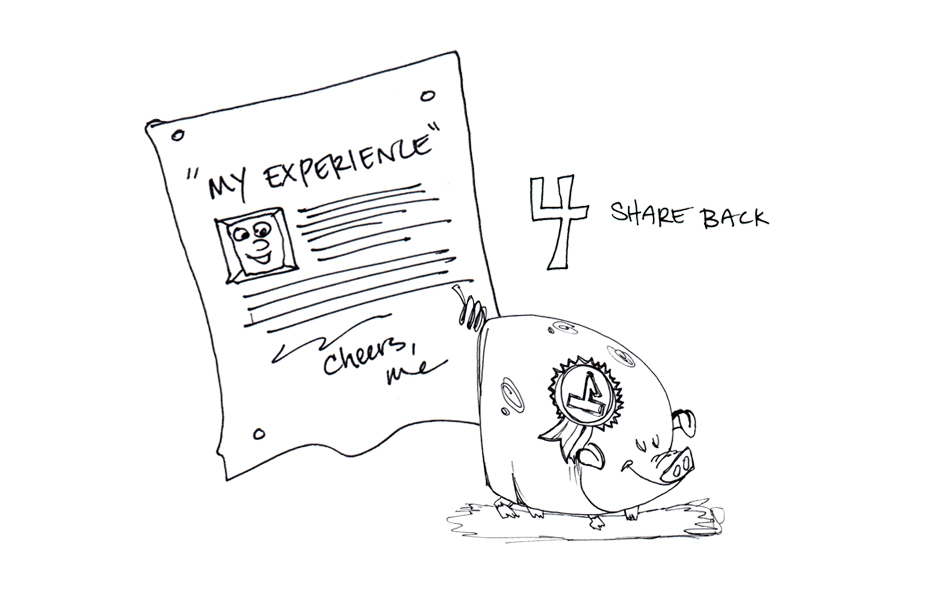
\includegraphics[width=.3\textwidth]{../pictures/OpenBook-2-4.jpg}}

\textbf{Wrap up the project with a critical assessment of progress and
directions for future work. Share any changes to this syllabus that you
think would be useful for future peeragogues!}

\emph{Activity} -- Identify the main obstacles you encountered. What are
some goals you were not able to accomplish yet? Did you foresee these
challenges at the outset? How did this project resemble or differ from
others you've worked on? How would you do things differently in future
projects? What would you like to tackle next?

\emph{Writing} -- Communicate your reflection case. Prepare a short
written or multimedia essay, dealing with your experiences in this
course. Share the results by posting it where others in the broader
Peeragogy project can find it.

\emph{`Extra credit'} -- Contribute back to one of the other
organisations or projects that helped you on this peeragogical journey.
Think about what you have to offer. Is it a bug fix, a constructive
critique, pictures, translation help, PR, wiki-gnoming or making a cake?
Make it something special, and people will remember you and thank you
for it.

\emph{Suggested resources} -- The Peeragogy Handbook, parts VIII
(`\href{http://peeragogy.org/resources/technologies/}{Technologies,
Services, and Platforms}') and IX
(`\href{http://peeragogy.org/resources/}{Resources}').

\emph{Recommended reading} -- Stallman, Richard.
``\href{http://www.gnu.org/philosophy/shouldbefree.html}{Why software
should be free}'' (1992).

\emph{Observations from the Peeragogy project} -- When we were deciding
how to license our work,~ we decided to use CC0, emphasizing~
`re-usability' and hoping that other people would come and remix the
handbook.~ At the moment, we're still waiting to see the first remix
edition, but we're confident that it will come along in due course.~
Maybe you'll be the one who makes it!

\subsection{{\tiny Micro-}Case Study: The Peeragogy Project, Year 1}

Since its conception in early 2012, the Peeragogy Project has collected
over 3700 comments in our discussion forum, and over 200 pages of
expository text in the handbook. It has given contributors a new way of
thinking about things together. However, the project has not had the
levels of engagement that should be possible, given the technology
available, the global interest in improving education, and the number of
thoughful participants who expressed interest. We hope that the handbook
and this accompanying syllabus will provide a seed for a new phase of
learning, with many new contributors and new ideas drawn from real-life
applications.

\subsection{{\tiny Micro-}Case Study: The Peeragogy Project, Year 2}

10 new handbook contributors joined in the project's second year. We've
begun a series of weekly Hangouts on Air that have brought in many
additional discussants, all key people who can help to fulfil
peeragogy's promise.~ The handbook has been considerably improved
through edits and discussion.~ The next step for us is putting this work
into action in the \emph{Peeragogy Accelerator}.

\subsection{{\tiny Micro-}Case Study: The Peeragogy Project, Year 3}

We published our plans as ``Building the Peeragogy Accelerator'',
presenting it at OER14 and inviting feedback.  In the run up to this,
we had been very active creating additional abstracts and submitting
them to conferences.  However, despite our efforts we failed to
recruit any newcomers for the trial run of the Accelerator.  Even so,
piloting the Accelerator with some of our own projects worked
reasonably well,\footnote{For an overview,
see \url{http://is.gd/up_peeragogy_accelerator}.} but we decided to
focus on the handbook in the second half of the year.  As the
project's line-up shifted, participants reaffirmed the importance of
having ``no camp counsellors.''  In the last quarter of 2014, we
created the workbook that is now presented in Part I, as a quickstart
guide to peeragogy.  We also revised the pattern catalog, and used the
revised format to create a ``distributed roadmap'' for the Peeragogy
project -- featured in Chapter \ref{distributed-roadmap} of the third
edition of the handbook.

% 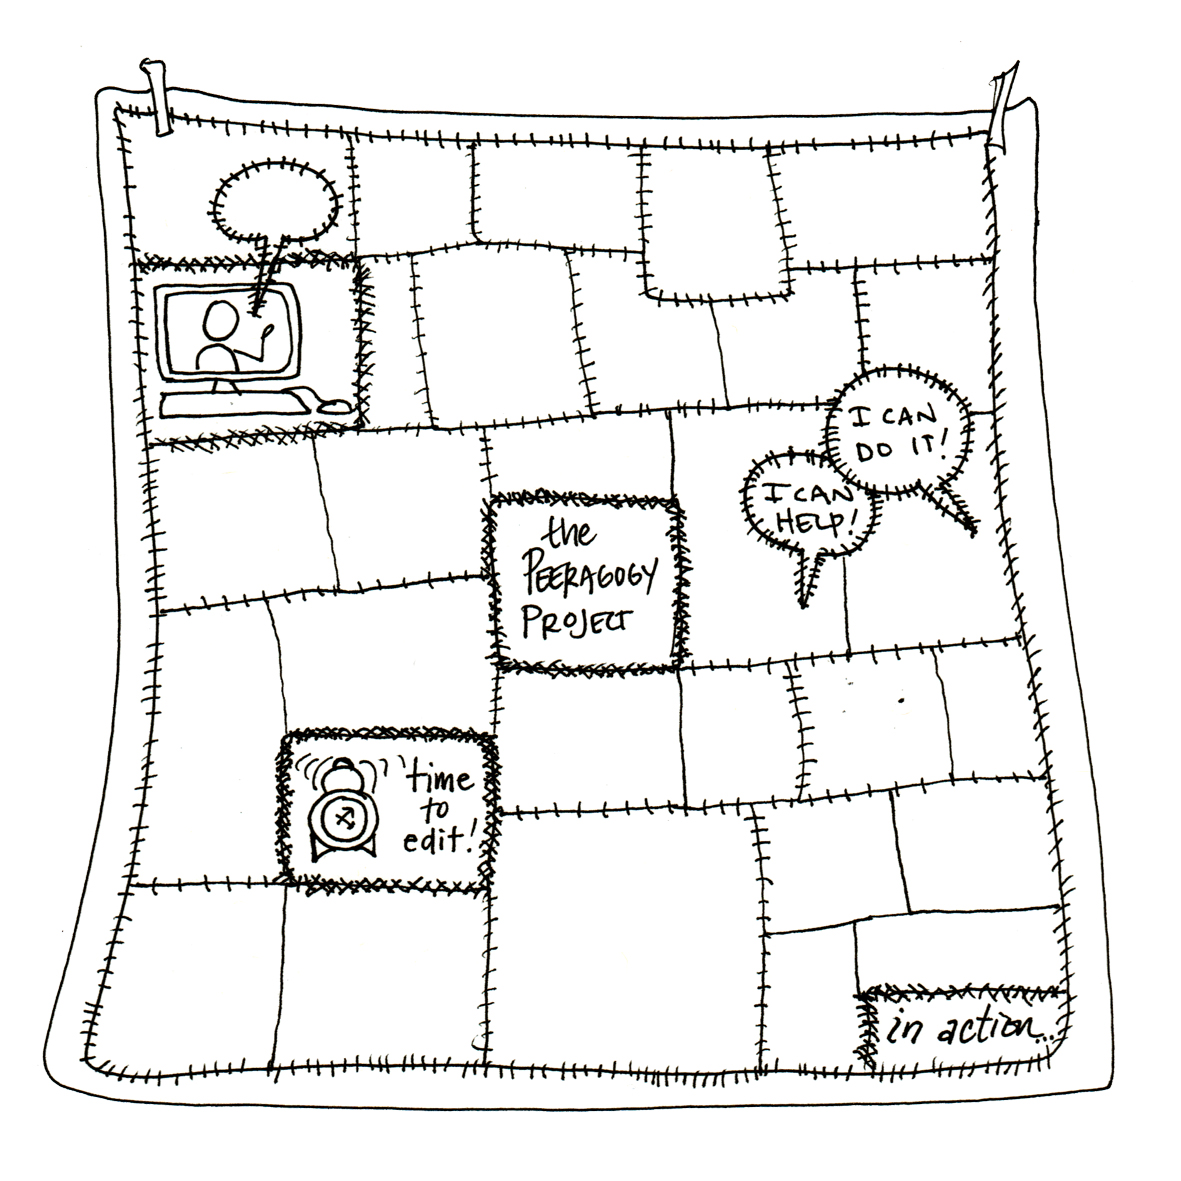
\includegraphics[width=.3\textwidth]{../pictures/OpenBook-3.jpg}
